\subsection{Критерий <<трёх сигм>>}

Для начала рассмотрим классический и основополагающий метод обнаружения аномалий с использованием критерия <<трех сигм>>. Этот метод является статистическим и основывается на предположении, что данные распределены нормально, и аномалии могут быть выявлены как те, которые выходят за пределы трех среднеквадратичных отклонений от среднего значения.

Из простоты метода следуют очевидные ограничения на область его применения: при значительном отклонении данных от распределения Гаусса эффективность и точность метода может значительно снизиться.

Для использования критерия необходимо рассчитать среднее значение и стандартное отклонение по формулам (\ref{average}) и (\ref{standard_deviation}) соответственно.

\begin{equation}\label{average}
    \mu = \frac{1}{n} \sum\limits_{i = 1}^{n}x_i,
\end{equation}

\begin{equation}\label{standard_deviation}
    \sigma = \sqrt{\frac{1}{n} \sum\limits_{i = 1}^{n}(x_i - \mu)^2},
\end{equation}
где $n$ – количество элементов выборки, $x_i$ --- $i$-ый элемент выборки.

Затем аномалии определяются как те значения, которые находятся за пределами интервала, определенного трех среднеквадратичных отклонений от среднего (см. рисунок~\ref{fig:three-sigma}).

\begin{figure}
  \centering
  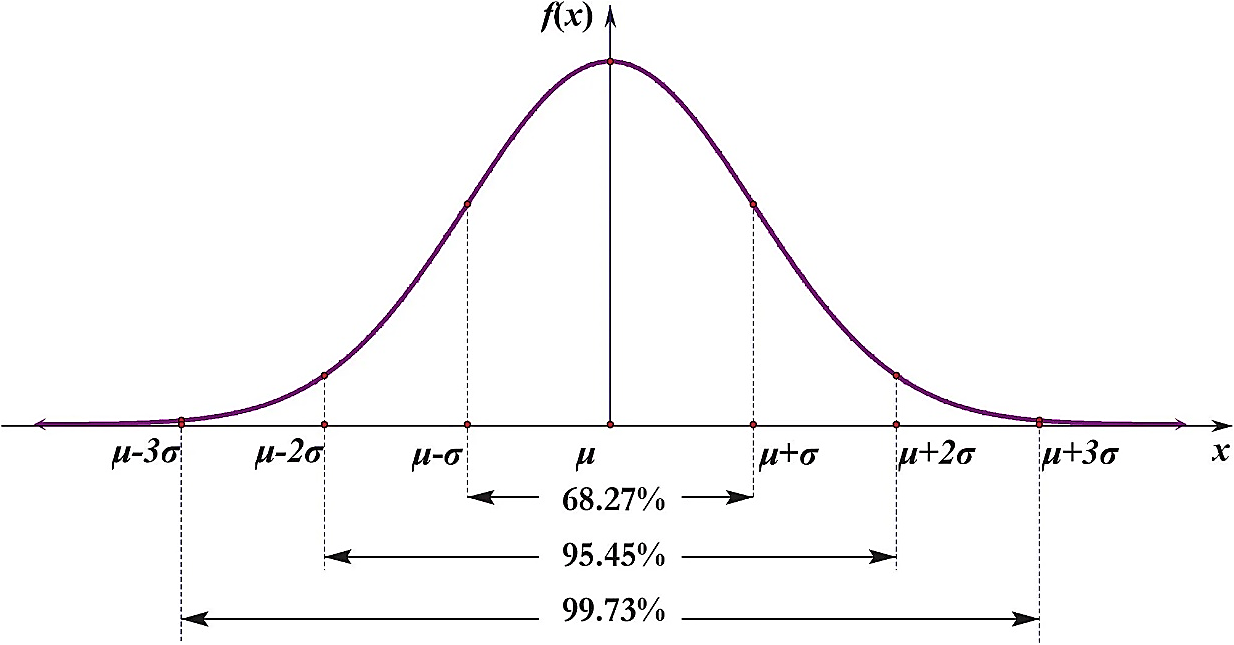
\includegraphics[scale=0.3]{inc/images/three-sigma.png}
  \caption{График нормального распределения и процент попадания в отрезки, равные среднеквадратичному отклонению \cite{Three-Sigma-Limits}}
  \label{fig:three-sigma}
\end{figure}

Помимо своей простоты, данный метод имеет ограничения в эффективности при обнаружении сложных нелинейных закономерностей в данных. Кроме того, такой подход не учитывает структуру данных и контекст анализа. Однако он включён рассмотрение ввиду его первоначальной каноничности для решения поставленной задачи. Многие статистические модели используют, развивают и усовершенствуют данный подход.

При использовании критерия <<трёх сигм>> формулируется функция принятия решения, которая непосредственно соответствует постановке задачи. В частности, определяем функцию (\ref{f_3sigma}):
\begin{equation}\label{f_3sigma}
    f(\overline{x_i}) = \begin{cases}
         \ \ 1, & \text{если } |\overline{x_i} - \mu| > 3\sigma, \\
        -1, & \text{если } |\overline{x_i} - \mu| \le 3\sigma,
    \end{cases}
\end{equation}
где $\mu$ и $\sigma$ вычисляются по формулам (\ref{average}) и (\ref{standard_deviation}). Таким образом, наблюдение $\overline{x_i}$ классифицируется как аномальное (метка $y_1$) при условии, что его отклонение от среднего превышает три стандартных отклонения.

\textit{При нормальном распределении признаков} вероятность ложноположительного срабатывания определяется выражением (\ref{alpha_3sigma}), а вероятность ошибки II-го рода --- соотношением (\ref{beta_3sigma}).
\begin{equation}\label{alpha_3sigma}
    \alpha = P\Big\{ |\overline{x_i} - \mu| > 3\sigma\ \Big|\ t_i\ -\ \text{«нормальный» экземпляр} \Big\},
\end{equation}

\begin{equation}\label{beta_3sigma}
    \beta = P\Big\{ |\overline{x_i} - \mu| \le 3\sigma\ \Big|\ t_i\ -\ \text{«аномальный» экземпляр} \Big\}.
\end{equation}
что удовлетворяет установленному ограничению $\alpha \leq p$, где порог $p$ выбран равным 0,05.

Таким образом метод, позволяет установить строгие границы для функции принятия решения $f$. При условии нормальности распределения данных, критерий <<трёх сигм>> обеспечивает очень малую вероятность ошибки I-го рода, что удовлетворяет ограничению, заданному в постановке задачи, и позволяет эффективно минимизировать $\beta$, что соответствует цели оптимизации, сформулированной в (\ref{task_formulation}). Однако сетевой трафик редко может быть описан распределением Гаусса, ввиду нерегулярности событий в вычислительных сетях, что даёт повод для рассмотрения других путей решения задачи.
